\section{C++ Quick Start}

\subsection{Object-Oriented Programming}

% 简单对比过程式编程和面向对象编程
\begin{frame}[fragile]{Procedural vs Object-Oriented Programming}
	\begin{columns}
		\begin{column}{0.5\textwidth}
			\textbf{C: Procedural Programming}
			\begin{itemize}
				\item Focus on functions and data
				\item Functions operate on data structures
				\item No built-in support for encapsulation or inheritance
			\end{itemize}
		\end{column}
		\begin{column}{0.5\textwidth}
			\textbf{C++: Object-Oriented Programming}
			\begin{itemize}
				\item Combines data and functions into classes
				\item Supports encapsulation, inheritance, and polymorphism
				\item Provides a more modular and reusable code structure
			\end{itemize}
		\end{column}
	\end{columns}

	A class defines a type \textbf{along with a collection of operations that are related to that type}.
\end{frame}

\begin{frame}[fragile]{Procedural vs Object-Oriented Programming}
	\begin{columns}
		\begin{column}{0.5\textwidth}
			\textbf{C Struct (Data \textcolor{orange}{and} Functions)}
			\begin{minted}{c}
struct Student {
    char name[50];
    int age;
    float gpa;
};
void print_student(struct Student s) {
    printf("Name: %s\n", s.name);
    printf("Age: %d\n", s.age);
    printf("GPA: %.2f\n", s.gpa);
}
int main() {
    struct Student alice = {"Alice", 20, 3.8};
    print_student(alice);
    return 0;
}
			\end{minted}
		\end{column}
		\begin{column}{0.5\textwidth}
			\textbf{C++ Class (Data \textcolor{orange}{with} Functions)}
			\begin{minted}{cpp}
class Student {
private:
    string name;
    int age;
    float gpa;
public:
    Student(string n, int a, float g)
        : name(n), age(a), gpa(g) {}
    void print() {
        cout << "Name: " << name << endl;
        cout << "Age: " << age << endl;
        cout << "GPA: " << gpa << endl;
    }
};
int main() {
    Student alice("Alice", 20, 3.8);
    alice.print();  // Object calls its own method
    return 0;
}
			\end{minted}
		\end{column}
	\end{columns}
\end{frame}

\begin{frame}[fragile]{Abstract Data Types}
	The fundamental ideas behind classes are \textbf{data abstraction} and \textbf{encapsulation}.

	\begin{itemize}
		\item \textbf{Data Abstraction}: Separation of \textcolor{blue}{interface} and \textcolor{orange}{implementation}
		\item \textbf{Encapsulation}: Enforces this separation by hiding implementation details
		\item Together, they define an \textbf{Abstract Data Type (ADT)}
	\end{itemize}

	\vspace{0.3em}
	\begin{columns}
		\begin{column}{0.5\textwidth}
			\textbf{Interface (What users see)}
			\begin{itemize}
				\item Public operations users can execute
				\item Contract of what the class does
				\item Think abstractly about behavior
			\end{itemize}
		\end{column}
		\begin{column}{0.5\textwidth}
			\textbf{Implementation (Hidden details)}
			\begin{itemize}
				\item Data members
				\item Function bodies
				\item Internal helper functions
			\end{itemize}
		\end{column}
	\end{columns}
\end{frame}

\begin{frame}[fragile]{Abstract Data Type: An Example}
	\begin{columns}
		\begin{column}{0.5\textwidth}
			\textbf{Interface (Public)}
			\begin{itemize}
				\item \texttt{Book(title, author, pages, count)} - Constructor
				\item \texttt{isAvailable()} - Check availability
				\item \texttt{addCopies(num)} - Add copies
			\end{itemize}
			\vspace{0.3em}
			\textbf{Users care about:} \\
			\textit{What} operations are available, not \textit{how} they work
		\end{column}
		\begin{column}{0.5\textwidth}
			\begin{minted}{cpp}
class Book {
private:  // Implementation (Hidden)
    string title;
    string author;
    int pages;
    int count;
public:   // Interface (Visible)
    Book(string t, string a, int p, int c);
    bool isAvailable() const;
    void addCopies(int num);
};
            \end{minted}
		\end{column}
	\end{columns}
\end{frame}

\begin{frame}[fragile]{Abstract Data Types: Key Benefits}

	\begin{columns}
		\begin{column}{0.5\textwidth}
			\textbf{For Class Designers:}
			\begin{itemize}
				\item Focus on \textbf{how} the class is implemented
				\item Can change implementation without breaking user code
				\item Control access to internal data
			\end{itemize}
		\end{column}
		\begin{column}{0.5\textwidth}
			\textbf{For Class Users:}
			\begin{itemize}
				\item Don't need to know \textbf{how} the type works
				\item Think abstractly about \textbf{what} the type does
				\item Use the interface without worrying about details
			\end{itemize}
		\end{column}
	\end{columns}
\end{frame}

\begin{frame}[fragile]{Class: Definition}
	\begin{minted}[fontsize=\scriptsize]{cpp}
class ClassName {
public:  // Public interface
    ClassName();  // Constructor
    ~ClassName(); // Destructor
    void publicMethod();  // Public method
private: // Private implementation details
    int privateData;  // Private data member
    void privateMethod();  // Private method
protected: // Protected members (accessible by derived classes)
    int protectedData;  // Protected data member
};
    \end{minted}
\end{frame}

% 介绍类的实例化
\begin{frame}[fragile]{Class: Instantiation}
	Instantiate a class to create an object
	\begin{itemize}
		\item Use the class name as a type
		\item Call the constructor to initialize the object
		\item Objects are instances of the class
	\end{itemize}
	\begin{minted}{cpp}
int main() {
    Point p(10, 20);  // Create an object of Point
    p.display();      // Call public method
    return 0;
}
    \end{minted}
\end{frame}

\begin{frame}[fragile]{Class: \texttt{this} pointer}
	A special pointer that refers to the current object

	\begin{itemize}
		\item Used inside class methods to access members of the current object
		\item Helps distinguish between member variables and parameters with the same name
	\end{itemize}

	\begin{minted}{cpp}
class Point {
private:
    int x, y;
public:
    Point(int x, int y) {
        this->x = x;  // Use this to refer to member variable
        this->y = y;  // Use this to refer to member variable
    }
};
    \end{minted}
\end{frame}

% 介绍右值引用
\begin{frame}[fragile]{Class: Rvalue References}
	\textbf{Rvalue Reference:} A new reference type introduced in C++11
	\begin{itemize}
		\item Allows binding to temporary objects (rvalues)
		\item Syntax: \texttt{Type\&\&} (double ampersand)
		\item Enables move semantics and perfect forwarding
	\end{itemize}

	\begin{minted}{cpp}
A& a_lref = a; // lvalue reference
A&& a_rref = a; // rvalue reference
	\end{minted}

    See: \textcolor{blue}{\href{https://www.open-std.org/jtc1/sc22/wg21/docs/papers/2006/n2027.html}{A Brief Introduction to Rvalue References - Bjarne Stroustrup}}
\end{frame}

% 介绍移动语义
\begin{frame}[fragile]{Class: Move Semantics}
	\begin{minted}{cpp}
template <class T> swap(T& a, T& b)
{
    T tmp(a);   // now we have two copies of a
    a = b;      // now we have two copies of b
    b = tmp;    // now we have two copies of tmp (aka a)
}

template <class T> swap(T& a, T& b) {
    T tmp = std::move(a);
    a = std::move(b);
    b = std::move(tmp);
}
    \end{minted}
\end{frame}

% 介绍 move()
\begin{frame}[fragile]{Class: \texttt{std::move}}
    \textbf{std::move:} A utility function that casts an object to an rvalue reference
    \begin{itemize}
        \item Indicates that the object can be moved
        \item Does not actually move anything, just changes the type
    \end{itemize}

    \textbf{Prototype:}
    \begin{minted}{cpp}
template <class T>
typename remove_reference<T>::type&&
move(T&& a)
{
    return a;
}
    \end{minted}
    It is now up to client code to overload key functions on whether their argument is an lvalue or rvalue.
\end{frame}

% 介绍拷贝
\begin{frame}[fragile]{Class: Copying Objects}
	C++ allows copying objects using the copy constructor
	\begin{itemize}
		\item Copy constructor: when an object is passed by value or returned from a function
		\item Default copy constructor performs a shallow copy (member-wise copy)
		\item Custom copy constructor can be defined for deep copying
	\end{itemize}

	\begin{columns}
		\begin{column}{0.5\textwidth}
			\begin{minted}{cpp}
class Point {
public:
    // Custom copy constructor
    Point(const Point& other) {
        x = other.x;
        y = other.y;
    }
};
\end{minted}
		\end{column}
		\begin{column}{0.5\textwidth}
			\begin{minted}{cpp}
Point p1(10, 20);
Point p2 = p1;  // Calls copy constructor
p2.display();   // Displays copied point
    \end{minted}
		\end{column}
	\end{columns}
\end{frame}

% 介绍移动
\begin{frame}[fragile]{Class: Moving Objects}
	C++11 introduced move semantics to optimize resource management
	\begin{itemize}
		\item Move constructor transfers ownership of resources from one object to another
		\item Avoids deep copying, improving performance for temporary objects
		\item Use \texttt{std::move} to indicate an object can be moved
	\end{itemize}

	\begin{columns}
		\begin{column}{0.5\textwidth}
			\begin{minted}{cpp}
class Point {
public:
    // Move constructor
    Point(Point&& other) noexcept {
        x = other.x;
        y = other.y;
        other.x = 0;  // Leave moved-from object in a valid state
        other.y = 0;
    }
};
\end{minted}
		\end{column}
		\begin{column}{0.5\textwidth}
			\begin{minted}{cpp}
Point p1(10, 20);
Point p2 = std::move(p1);  // Calls move constructor
p2.display();               // Displays moved point
            \end{minted}
		\end{column}
	\end{columns}
\end{frame}


% 介绍析构
\begin{frame}[fragile]{Class: Destructor}
	\textbf{Destructor:} A special member function called when an object goes out of scope or is deleted
	\begin{itemize}
		\item Cleans up resources (memory, file handles, etc.)
		\item Automatically called when the object is destroyed
		\item Can be defined to perform custom cleanup actions
	\end{itemize}

    \begin{columns}
        \begin{column}{0.5\textwidth}
	\begin{minted}{cpp}
class Point {
public:
    // Destructor
    ~Point() {
        cout << "Point(" << x << ", " << y << ") destroyed" << endl;
    }
};
        \end{minted}
        \end{column}
        \begin{column}{0.5\textwidth}
                    \begin{minted}{cpp}
int main() {
    Point p(10, 20);  // Constructor called
    p.display();      // Displays point
    return 0;        // Destructor called automatically
}
    \end{minted}
    \end{column}
    \end{columns}
\end{frame}



\begin{frame}[fragile]{Encapsulation}
	\textbf{Encapsulation enforces the separation of interface and implementation}
	\begin{itemize}
		\item \textbf{Hide Implementation}: Users cannot access internal details
		\item \textbf{Control Access}: Define exactly how others can use your class
		\item \textbf{Maintainability}: Change implementation without breaking user code
		\item \textbf{Data Protection}: Prevent accidental or malicious modification
	\end{itemize}

\end{frame}

\begin{frame}[fragile]{Encapsulation: Access specifiers}
	\begin{minted}[fontsize=\scriptsize]{cpp}
class BankAccount {
private:    // Only this class can access
    double balance;
public:     // Anyone can access
    void deposit(double amount) {
        if (amount > 0) balance += amount;  // Safe deposit
    }
    double getBalance() const { return balance; }  // Read-only access
protected:  // This class and its children can access
    void setBalance(double newBalance) { balance = newBalance; }
};
    \end{minted}
	\begin{itemize}
		\item \texttt{struct}: Members are \textbf{public} by default - less encapsulation
		\item \texttt{class}: Members are \textbf{private} by default - enforces encapsulation
	\end{itemize}
\end{frame}

\begin{frame}[fragile]{Inheritance: Building on Existing Code}
	\textbf{Like a Family Tree:} Children inherit traits from parents

	\begin{columns}
		\begin{column}{0.3\textwidth}
			\textbf{Base Class (Parent)}
			\begin{minted}{cpp}
class Animal {
protected:
    string name;
public:
    Animal(string n) : name(n) {}
    void eat() { cout << name << " is eating\n"; }
    virtual void makeSound() { cout << name << " makes a sound\n"; }
};
    \end{minted}
		\end{column}
		\begin{column}{0.7\textwidth}
			\textbf{Derived Class (Child)}
			\begin{minted}{cpp}
class Dog : public Animal {
public:
    Dog(string n) : Animal(n) {}  // Call parent constructor
    void makeSound() override {        // Override parent method
        cout << name << " barks: Woof!\n";
    }
    void wagTail() { cout << name << " wags tail\n"; }  // New method
};

int main() {
    Dog buddy("Buddy");
    buddy.eat();        // Inherited from Animal
    buddy.makeSound();  // Dog's own version
    buddy.wagTail();    // Dog-specific behavior
    return 0;
}
    \end{minted}
		\end{column}
	\end{columns}
\end{frame}

\begin{frame}[fragile]{Polymorphism: One Interface, Many Forms}
	\textbf{Like a Universal Remote:} Same buttons, different devices

	\begin{columns}
		\begin{column}{0.6\textwidth}
			\begin{minted}{cpp}
class Shape {
public:
    virtual double area() = 0;  // Pure virtual function
    virtual ~Shape() = default;
};
class Circle : public Shape {
    double radius;
public:
    Circle(double r) : radius(r) {}
    double area() override { return 3.14159 * radius * radius; }
};
class Rectangle : public Shape {
    double width, height;
public:
    Rectangle(double w, double h) : width(w), height(h) {}
    double area() override { return width * height; }
};
    \end{minted}
		\end{column}
		\begin{column}{0.4\textwidth}

			\begin{minted}{cpp}
vector<unique_ptr<Shape>> shapes;
shapes.push_back(make_unique<Circle>(5.0));
shapes.push_back(
    make_unique<Rectangle>(4.0, 6.0));
for (auto& shape : shapes) {
    cout << "Area: " << shape->area()
         << endl;
    // Calls correct method
}
    \end{minted}
		\end{column}
	\end{columns}
\end{frame}

\subsection{The Basics}

\begin{frame}[fragile]{I/O Streams: Compared to C Standard I/O}
	\begin{columns}
		\begin{column}{0.5\textwidth}
			\textbf{C Style}
			\begin{minted}{c}
#include <stdio.h>
#include <stdlib.h>

void print_msg(void) {
    printf("Hello from C!\n");
}

int main() {
    FILE* fp = fopen("test.txt", "r");
    if (fp) {
        // Manual resource management
        char line[100];
        while (fgets(line, 100, fp) != NULL) {
            printf("%s", line);
        }
        fclose(fp);
    }
    return 0;
}
			\end{minted}
		\end{column}
		\begin{column}{0.5\textwidth}
			\textbf{C++ Style}
			\begin{minted}{cpp}
#include <iostream>
#include <fstream>

void print_msg() {
    std::cout << "Hello from C++!" << std::endl;
}

int main() {
    std::ifstream file("test.txt");
    if (file.is_open()) {
        // Automatic resource management
        std::string line;
        while (std::getline(file, line)) {
            std::cout << line << std::endl;
        }
    }
    return 0;
}
			\end{minted}
		\end{column}
	\end{columns}
\end{frame}

% 介绍 C++ 的引用和指针
\begin{frame}[fragile]{References}
	\begin{columns}
		\begin{column}{0.5\textwidth}
			\textbf{C Pointers}
			\begin{minted}{c}
void swap_c(int* a, int* b) {
    int temp = *a;
    *a = *b;
    *b = temp;
}
int main() {
    int x = 5, y = 10;
    swap_c(&x, &y);  // Pass addresses
    printf("x=%d, y=%d\n", x, y);
    return 0;
}
			\end{minted}
		\end{column}
		\begin{column}{0.5\textwidth}
			\textbf{C++ References}
			\begin{minted}{cpp}
void swap_cpp(int& a, int& b) {
    int temp = a;
    a = b;
    b = temp;
}
int main() {
    int x = 5, y = 10;
    swap_cpp(x, y);  // Direct pass
    cout << "x=" << x << ", y=" << y << endl;
    return 0;
}
			\end{minted}
		\end{column}
	\end{columns}

	\vspace{0.5em}
	\begin{itemize}
		\item References are \textbf{aliases} for existing objects: \texttt{int a; int\& b = a;}
		\item References must be initialized and cannot be reassigned
	\end{itemize}
\end{frame}

% 本页展示 C++ 的所有运算符
\begin{frame}[fragile]{C++ Operators and Keywords (From \textcolor{blue}{\href{https://en.cppreference.com/w/cpp/language/}{cppreference.com}})}
	\begin{columns}
		\begin{column}{0.6\textwidth}
			\begin{figure}
				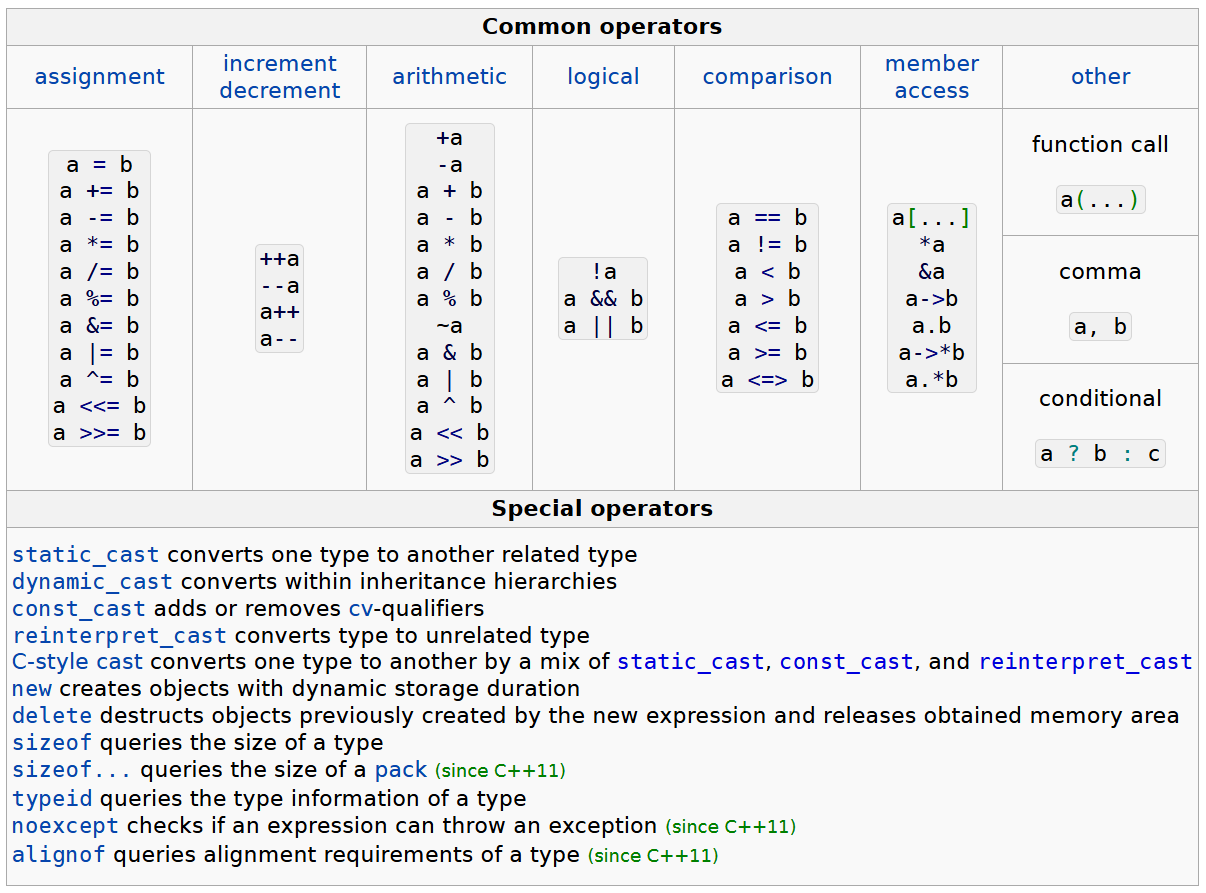
\includegraphics[width=\textwidth]{day8_pm/img/1-operators}
			\end{figure}
		\end{column}
		\begin{column}{0.4\textwidth}
			\begin{figure}
				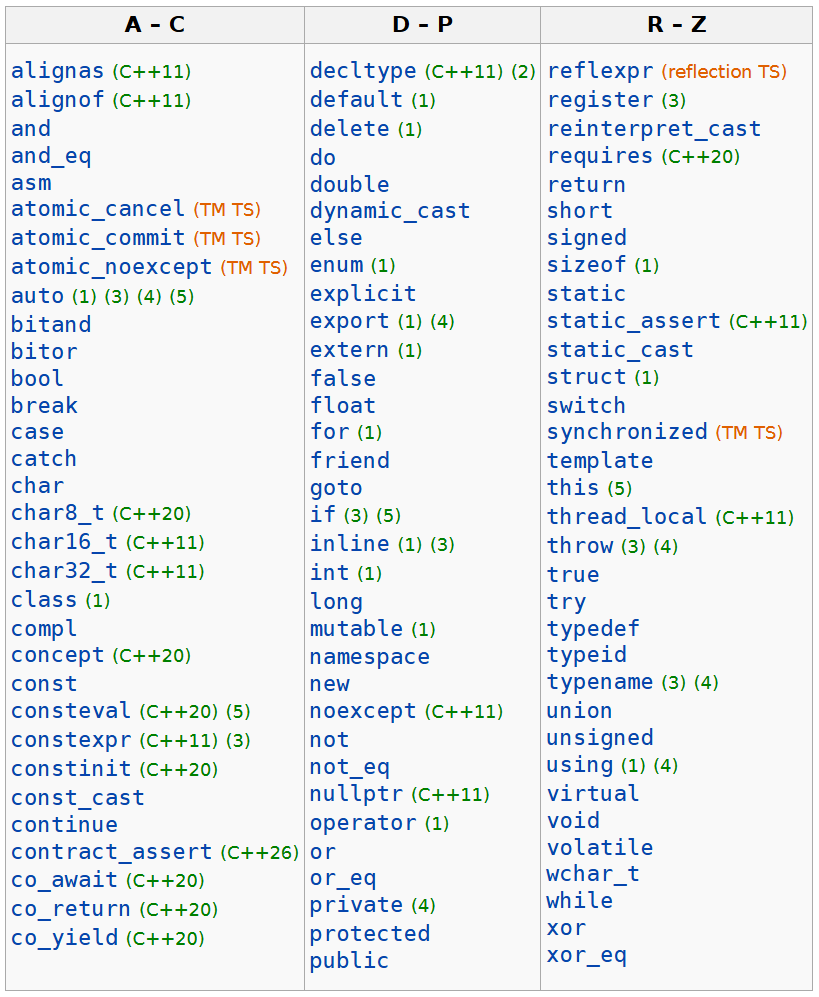
\includegraphics[width=0.9\textwidth]{day8_pm/img/1-keywords}
			\end{figure}
		\end{column}
	\end{columns}
\end{frame}

\begin{frame}[fragile]{C++ Operators and Keywords}
	We'll meet some new friends in this class:
	\begin{itemize}
		\item \textbf{I/O}:  \texttt{>>}, \texttt{<<}
		\item \textbf{Memory}: \texttt{new}, \texttt{delete}, \texttt{new[]}, \texttt{delete[]}
		\item \textbf{Type System}: \texttt{auto}, \texttt{decltype}, \texttt{using}, \texttt{operator}
		\item \textbf{Class}: \texttt{::}, \texttt{public}, \texttt{private}, \texttt{protected}, \texttt{friend}, \texttt{virtual}, \texttt{override}, \texttt{final}
	\end{itemize}
\end{frame}

% 上页给出代码对比,本页给出讲解
\begin{frame}[fragile]{I/O Streams}
	\begin{table}[]
		% table of streams: i, o, io; file, string, c
		\begin{tabular}{cccc}
			\hline
			\textbf{Type} & \textbf{Input}         & \textbf{Output}                             & \textbf{Both}         \\ \hline
			standard      & \texttt{cin}           & \texttt{cout}, \texttt{cerr}, \texttt{clog} &                       \\ \hline
			File          & \texttt{ifstream}      & \texttt{ofstream}                           & \texttt{fstream}      \\ \hline
			String        & \texttt{istringstream} & \texttt{ostringstream}                      & \texttt{stringstream} \\ \hline
		\end{tabular}
	\end{table}

	\textbf{Benefits of C++ Streams:}
	\begin{itemize}
		\item Type safety and flexibility
		\item Easier to read and maintain code
		\item Automatic resource cleanup when objects go out of scope
	\end{itemize}
\end{frame}

% 给出一个 sstream 的例子,以展示相比 C 的优势
\begin{frame}[fragile]{I/O Streams: Example}
	\textbf{String Streams:} Like a string that can be read/written like a file
	\begin{minted}{cpp}
#include <sstream>
#include <iostream>

void example_string_stream() {
    std::stringstream ss;
    ss << "The answer is " << 42;
    std::string result = ss.str();
    std::cout << result << std::endl;
}
    \end{minted}

	\textbf{Benefits:}
	\begin{itemize}
		\item Concise syntax for formatting strings
		\item No need for manual memory management
		\item Can be used with any type that supports stream operators
	\end{itemize}
\end{frame}

% 介绍命名空间,标准库的所有名字都在命名空间 std 中
\begin{frame}[fragile]{Namespaces}
	\begin{itemize}
		\item C++ uses namespaces to avoid \textbf{name collisions}
		\item \textbf{Standard library} functions and classes are in the \texttt{std} namespace
		\item Use \texttt{using namespace std;} to avoid prefixing with \texttt{std::} (should be avoided in header files and large projects)
	\end{itemize}
	\textbf{Example:}
	\begin{minted}[fontsize=\scriptsize]{cpp}
#include <iostream>
using namespace std;
cout << "Hello, World!" << endl;
        \end{minted}
\end{frame}

% 介绍运算符语法
\begin{frame}[fragile]{Class: Operator overloading}
	\begin{itemize}
		\item C++ lets us define what the operators mean \textbf{when applied to objects of class type}.
		\item They are \textbf{special functions} with concise syntax
		\item Can be \textbf{overloaded} to provide custom behavior for user-defined types
		\item In a user-defined operator overload, \textbf{any type} can be used as return type (including \texttt{void})
		\item Operators for \textbf{primitive types} like \texttt{int}, \texttt{float}, etc. cannot be overloaded
	\end{itemize}

	\textbf{Syntax:}
	\begin{minted}[fontsize=\scriptsize]{cpp}
<return_type> operator<operator_symbol>(<parameters>) { /* Implementation */ }
// An illustration of overloading the + operator
int operator+(int a, int b) { return a + b; }
    \end{minted}
\end{frame}

% 以 I/O 操作符为例,介绍运算符重载:巧妙地通过重载,利用了移位运算符的语法
\begin{frame}[fragile]{Class: Operator overloading}
	\textbf{Why Overload I/O Operators?}
	\begin{itemize}
		\item Makes it easy to print custom objects
		\item Uses existing syntax (\texttt{<<} and \texttt{>>}) for a natural feel
	\end{itemize}

	\textbf{Prototype}
	% A prototype demonstrating how stream class overloads the I/O operators
	\begin{minted}{cpp}
template< class Traits >
basic_ostream<char, Traits>&
    operator<<( basic_ostream<char, Traits>& os, const char* s );
basic_istream& operator>>( int& value );
    \end{minted}
	\textbf{Example Usage}:
	\begin{minted}{cpp}
cout << "Hello, World!" << endl;
cin >> user_input;
    \end{minted}
\end{frame}

\begin{frame}[fragile]{Function Overloading: Same Name, Different Parameters}
	\textbf{Function Overloading:} Multiple functions with the same name but different parameters

	\begin{itemize}
		\item C++ allows multiple functions with the same name
		\item Functions must differ in number or type of parameters
		\item Compiler chooses the best match based on arguments
		\item Return type alone is \textbf{not} enough to distinguish functions
	\end{itemize}
\end{frame}

\begin{frame}[fragile]{Function Overloading vs C Naming Conventions}
	\begin{columns}
		\begin{column}{0.5\textwidth}
			\textbf{C Style: Different Names}
			\begin{minted}[fontsize=\tiny]{c}
#include <stdio.h>
#include <math.h>

// Need different names for each type
int abs_int(int x) { return x < 0 ? -x : x; }
double abs_double(double x) { return x < 0.0 ? -x : x; }
float abs_float(float x) { return x < 0.0f ? -x : x; }
int main() {
    printf("%d\n", abs_int(-5));
    printf("%.2f\n", abs_double(-3.14));
    printf("%.2f\n", abs_float(-2.5f));
    return 0;
}
            \end{minted}
		\end{column}
		\begin{column}{0.5\textwidth}
			\textbf{C++ Style: Overloaded Functions}
			\begin{minted}[fontsize=\tiny]{cpp}
#include <iostream>
#include <cmath>
using namespace std;
// Same name, different parameters
int abs(int x) { return x < 0 ? -x : x; }
double abs(double x) { return x < 0.0 ? -x : x; }
float abs(float x) { return x < 0.0f ? -x : x; }

int main() {
    cout << abs(-5) << endl;   // Calls abs(int)
    cout << abs(-3.14) << endl;// Calls abs(doubl)
    cout << abs(-2.5f) << endl;// Calls abs(float)
    return 0;
}
            \end{minted}
		\end{column}
	\end{columns}
\end{frame}

\begin{frame}[fragile]{Function Overloading: Rules and Best Practices}
	\textbf{Overloading Rules:}
	\begin{itemize}
		\item Functions must differ in \textbf{number} or \textbf{type} of parameters
		\item \textbf{const} and non-const parameters are considered different
		\item Reference and non-reference parameters are different
		\item Return type alone cannot distinguish overloaded functions
	\end{itemize}

	\textbf{Example of Valid Overloads:}
	\begin{minted}[fontsize=\scriptsize]{cpp}
void func(int x);                    // Version 1
void func(double x);                 // Version 2: different type
void func(int x, int y);             // Version 3: different number of para
void func(const int& x);             // Version 4: different parameter form
// void func(int x) { return 5; }    // ERROR: Only return type differs
    \end{minted}

	\textbf{Best Practice:} Use overloading for functions that perform \textbf{similar operations} on different types
\end{frame}

\subsection{Containers and Algorithms}
\begin{frame}[fragile]{STL: Your Programming Toolbox}
	\textbf{Standard Template Library (STL):}
	\begin{itemize}
		\item \textbf{Containers}: Ready-made data structures (like toolboxes)
		\item \textbf{Algorithms}: Common operations (like tools)
		\item \textbf{Iterators}: Ways to access container elements (like handles)
	\end{itemize}

	\vspace{0.5em}
	\textbf{Why use STL instead of arrays?}
	\begin{itemize}
		\item \textbf{Safety}: Automatic bounds checking and memory management
		\item \textbf{Convenience}: Built-in functions for common operations
		\item \textbf{Performance}: Optimized implementations
		\item \textbf{Compatibility}: Works seamlessly with C++ features
	\end{itemize}
\end{frame}

\begin{frame}[fragile]{Common Containers: Your Data Storage Options}
	\begin{columns}
		\begin{column}{0.5\textwidth}
			\textbf{Vector: Dynamic Array}
			\begin{minted}{cpp}
vector<int> numbers;
// Add elements
numbers.push_back(10);
numbers.push_back(20);
numbers.push_back(30);
// Access elements
cout << "First: " << numbers[0] << endl;
cout << "Size: " << numbers.size() << endl;
// Iterate through all
for (int num : numbers) { cout << num << " "; }
			\end{minted}
		\end{column}
		\begin{column}{0.5\textwidth}
			\textbf{Map: Key-Value Storage}
			\begin{minted}{cpp}
map<string, int> scores;
// Add key-value pairs
scores["Alice"] = 95;
scores["Bob"] = 87;
scores["Charlie"] = 92;
// Look up values
cout << "Alice's score: "
            << scores["Alice"] << endl;
// Check if key exists
if (scores.find("David") != scores.end()) {
    cout << "David found\n";
} else {
    cout << "David not found\n";
}
			\end{minted}
		\end{column}
	\end{columns}
\end{frame}

\begin{frame}[fragile]{Algorithms: Ready-Made Solutions}
	\textbf{Common algorithms you'll use:}
	\begin{table}[]
		\begin{tabular}{|l|l|}
			\hline
			\textbf{Category}       & \textbf{Algorithms}                                                                  \\ \hline
			\textbf{Sorting}        & \texttt{sort}, \texttt{stable\_sort}, \texttt{partial\_sort}, \texttt{nth\_element}  \\ \hline
			\textbf{Searching}      & \texttt{find}, \texttt{binary\_search}, \texttt{lower\_bound}, \texttt{upper\_bound} \\ \hline
			\textbf{Modifying}      & \texttt{copy}, \texttt{swap}, \texttt{replace}, \texttt{fill}, \texttt{transform}    \\ \hline
			\textbf{Set Operations} & \texttt{set\_union}, \texttt{set\_intersection}, \texttt{set\_difference}            \\ \hline
			\textbf{Numeric}        & \texttt{accumulate}, \texttt{inner\_product}, \texttt{adjacent\_difference}          \\ \hline
		\end{tabular}
	\end{table}
\end{frame}

\begin{frame}[fragile]{Algorithms: Ready-Made Solutions}
	\begin{minted}[fontsize=\scriptsize]{cpp}
vector<int> numbers = {64, 34, 25, 12, 22, 11, 90};
// Sort the vector
sort(numbers.begin(), numbers.end());
cout << "Sorted: ";
for (int n : numbers) cout << n << " ";
cout << endl;
// Find an element
auto it = find(numbers.begin(), numbers.end(), 25);
if (it != numbers.end()) {
    cout << "Found 25 at position: "
                << (it - numbers.begin()) << endl;
}
// Count elements greater than 30
int count = count_if(numbers.begin(), numbers.end(),
    [](int n) { return n > 30; });
cout << "Numbers > 30: " << count << endl;
    \end{minted}
\end{frame}

\begin{frame}[fragile]{More on STL Algorithms}
	\begin{figure}
		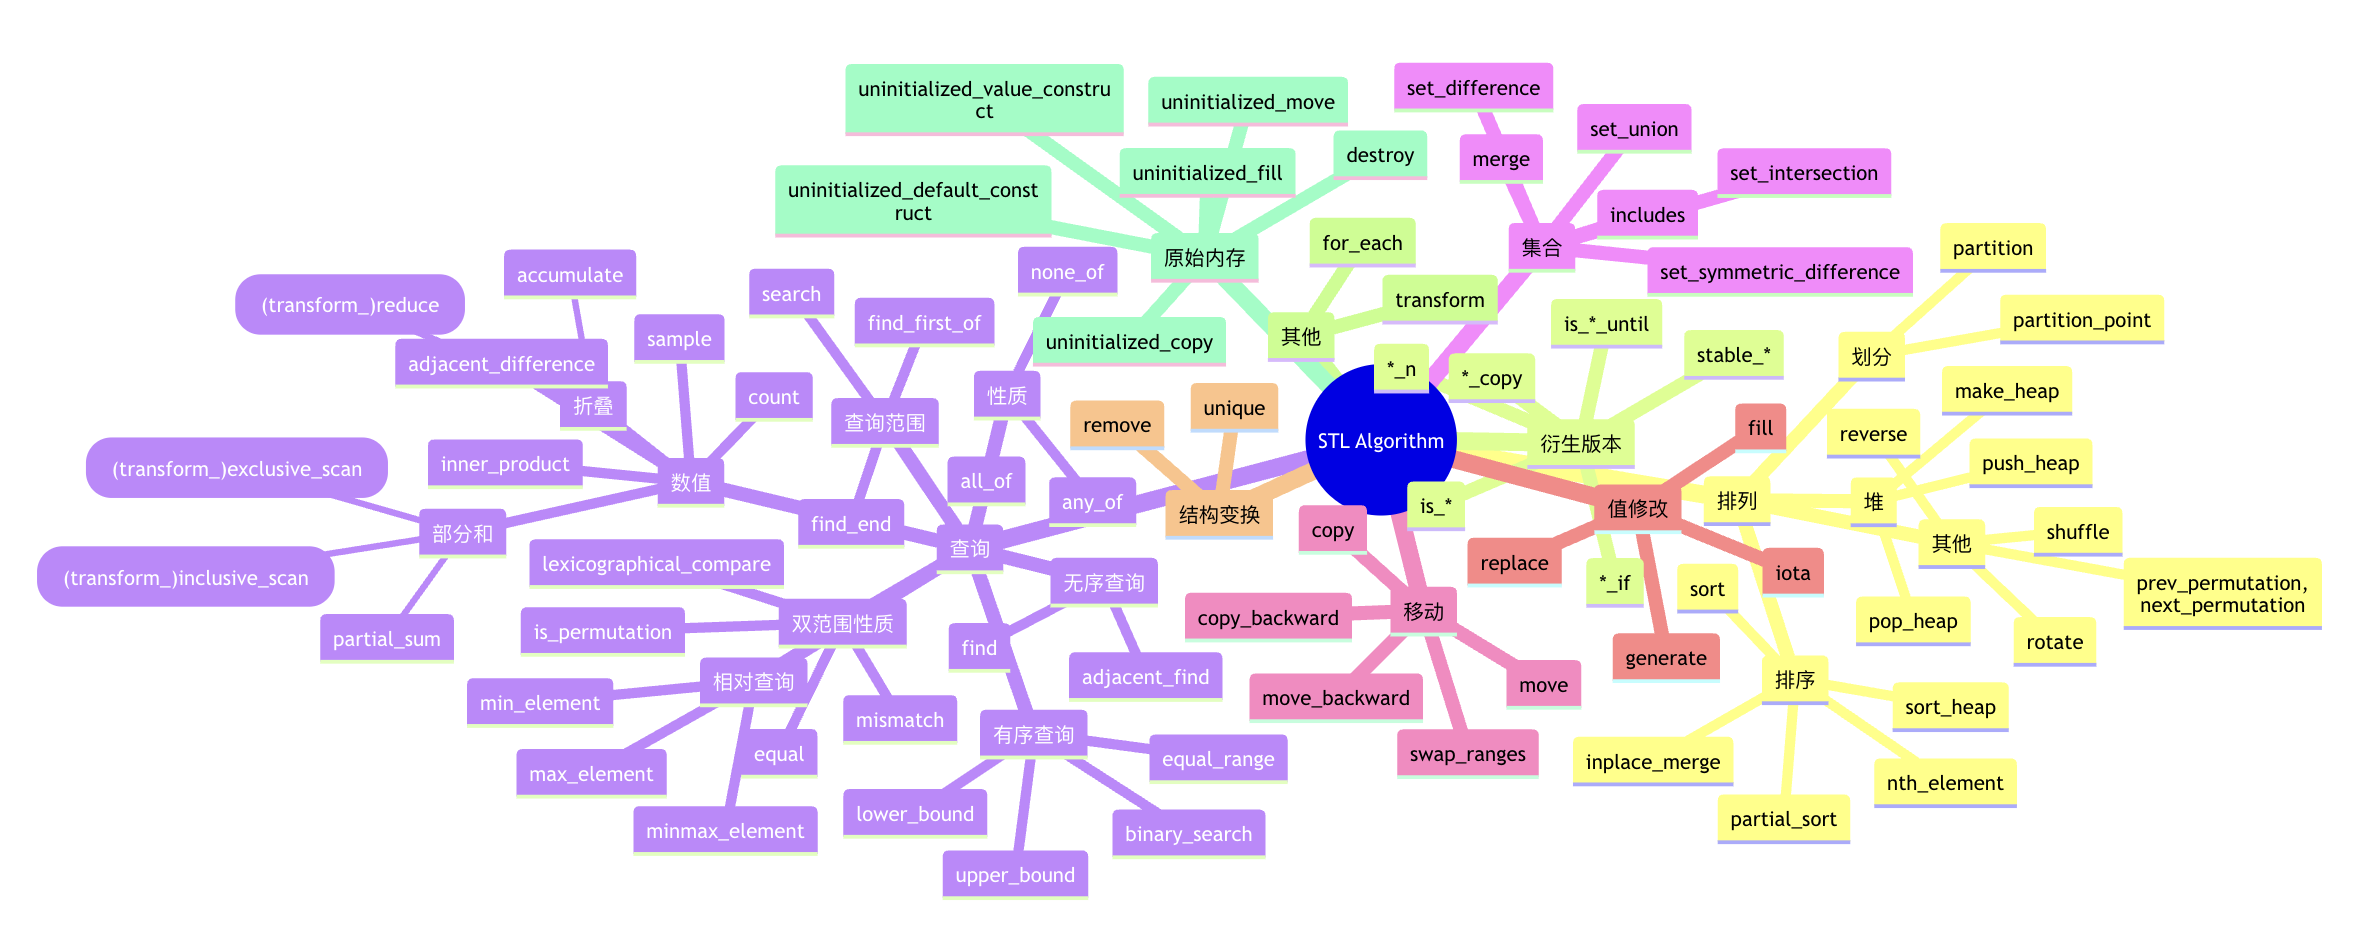
\includegraphics[width=\textwidth]{day8_pm/img/2-algorithms}
	\end{figure}
\end{frame}

\begin{frame}[fragile]{More on STL Algorithms}
	\textcolor{blue}{\href{https://www.youtube.com/watch?v=2olsGf6JIkU&ab_channel=CppCon}{CppCon 2018: 105 STL Algorithms in Less Than an Hour}}
	\begin{figure}
		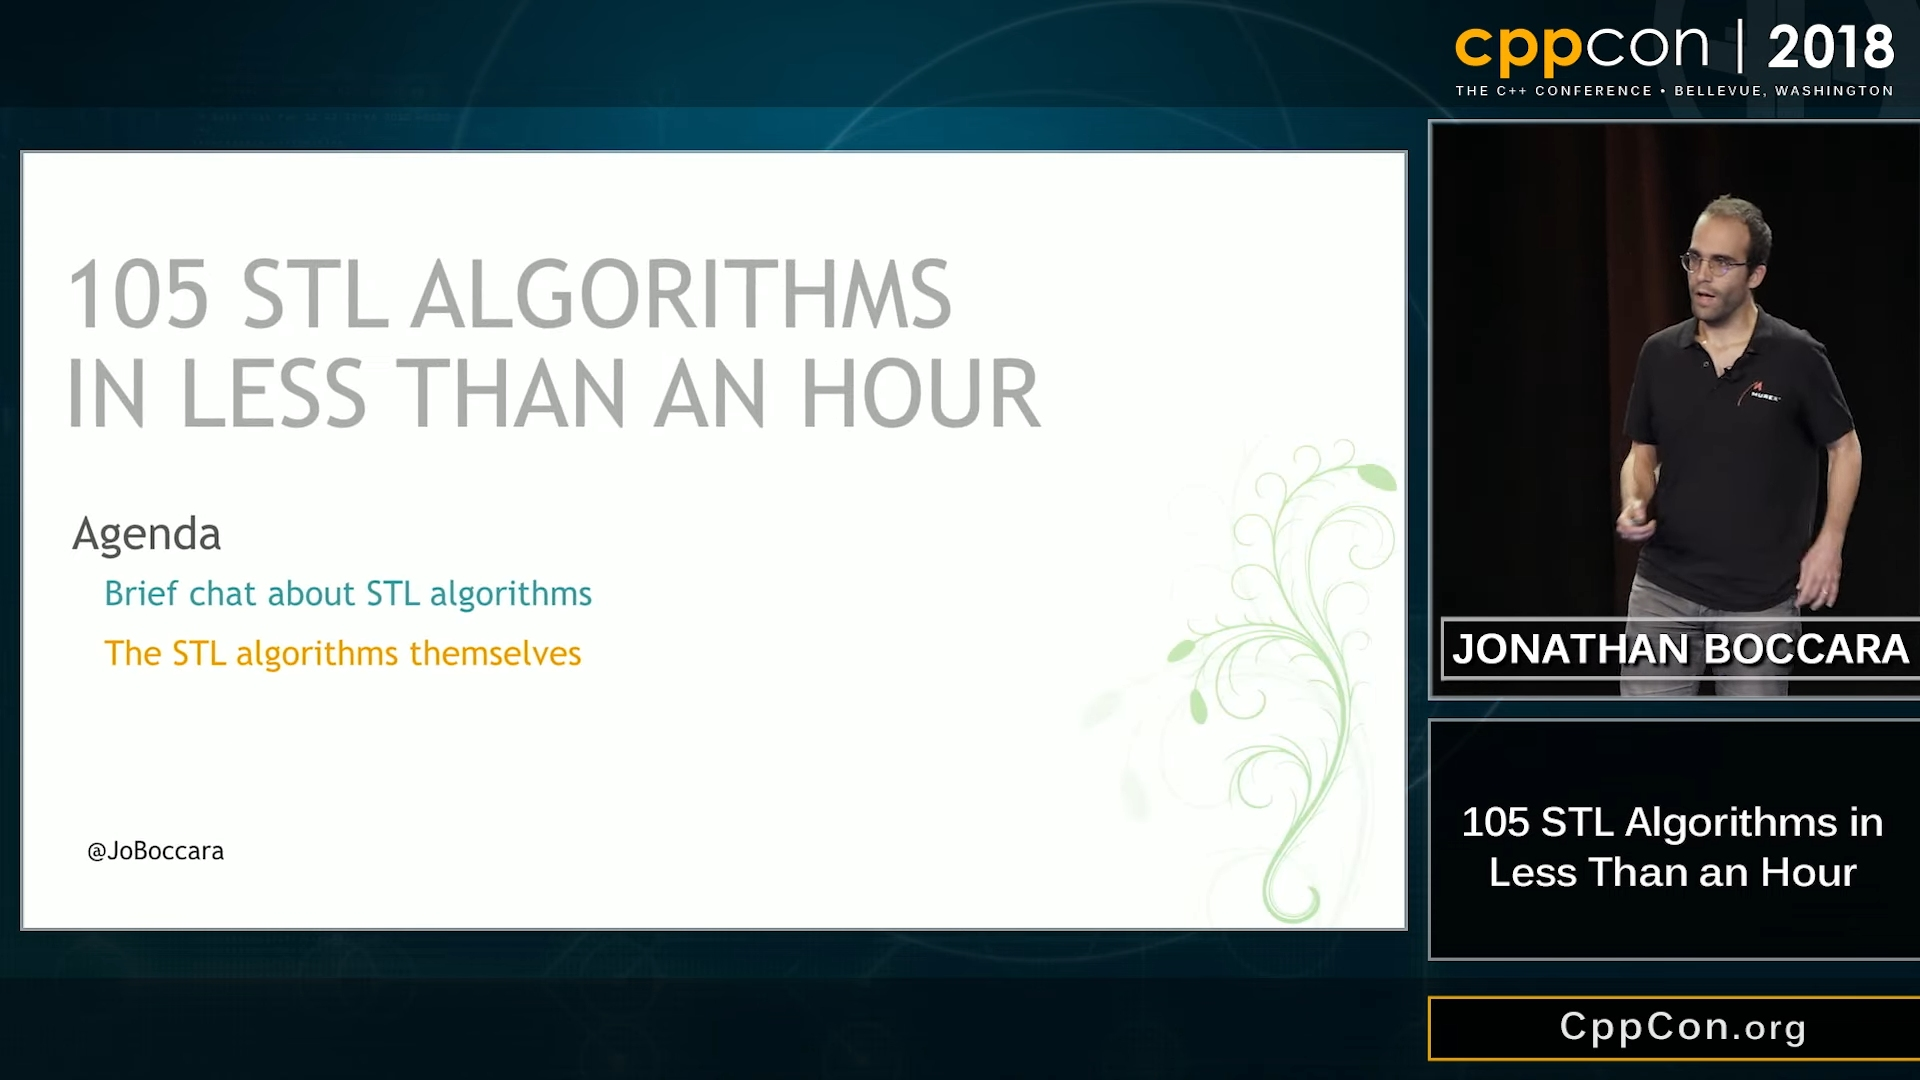
\includegraphics[width=0.7\textwidth]{day8_pm/img/2-cppcon2018}
	\end{figure}
\end{frame}

\begin{frame}[fragile]{Containers vs C Arrays: The Upgrade}
	\begin{columns}
		\begin{column}{0.5\textwidth}
			\textbf{C Arrays (Manual Everything)}
			\begin{minted}{c}
int arr[] = {1, 3, 2};
int size = 0;
// must write your compare function
qsort(ints, size, sizeof(int), compare_ints);
for (int i = 0; i < size; i++) {
    printf("%d ", arr[i]);
}
			\end{minted}
		\end{column}
		\begin{column}{0.5\textwidth}
			\textbf{C++ Containers (Automatic)}
			\begin{minted}{cpp}
// Dynamic size, automatic memory
vector<int> arr = {1, 3, 2};
sort(arr.begin(), arr.end());
for (int num : arr) {
    cout << num << " ";
}
			\end{minted}
		\end{column}
	\end{columns}

	\vspace{0.5em}
	\textbf{Benefits:} Safer, shorter, and often faster code!
\end{frame}

\subsection{Essential Features for Concurrency}
\begin{frame}[fragile]{Callable Objects}
	\textbf{Function Call Operator}
	\begin{minted}{cpp}
function (arg1, arg2, arg3,...)
    \end{minted}

	\textbf{Callable Object}
	\begin{itemize}
		\item An object that can be called like a function
		\item Functions and pointers to functions, \textbf{lambdas}, objects created by bind, and \textbf{classes that overload the function-call operator}.
	\end{itemize}
\end{frame}

\begin{frame}[fragile]{Lambda Expressions: The Core of Thread Functions}
	\begin{columns}
		\begin{column}{0.5\textwidth}
			\textbf{C Function Pointers}
			\begin{minted}{c}
#include <pthread.h>

void* thread_func(void* arg) {
    int id = *(int*)arg;
    printf("Thread %d running\n", id);
    return NULL;
}

int main() {
    pthread_t thread;
    int id = 1;
    pthread_create(&thread, NULL,
                   thread_func, &id);
    pthread_join(thread, NULL);
    return 0;
}
			\end{minted}
		\end{column}
		\begin{column}{0.5\textwidth}
			\textbf{C++ Lambda}
			\begin{minted}{cpp}
#include <thread>
#include <iostream>

int main() {
    int id = 1;

    // Lambda expression
    auto thread_func = [id]() {
        cout << "Thread " << id
                  << " running" << endl;
    };

    thread t(thread_func);
    t.join();

    return 0;
}
			\end{minted}
		\end{column}
	\end{columns}

\end{frame}

\begin{frame}[fragile]{Lambda Expressions: Syntax}
	\begin{minted}{cpp}
auto lambda_name = [capture](parameters) -> return_type {
    // function body
};
    \end{minted}
	\textbf{Example:}
	\begin{minted}{cpp}
auto add = [](int a, int b) -> int {
    return a + b;
};
cout << "Sum: " << add(3, 4) << endl; // Outputs 7
    \end{minted}
\end{frame}

\begin{frame}[fragile]{Lambda Expressions: Capture Clause}
	\begin{itemize}
		\item \texttt{[capture]}: How to access variables from the surrounding scope
		\item \texttt{[=]}: Capture all by value
		\item \texttt{[\&]}: Capture all by reference
		\item \texttt{[id]}: Capture specific variable by value
		\item \texttt{[\&id]}: Capture specific variable by reference
	\end{itemize}
\end{frame}

\begin{frame}[fragile]{Smart Pointers vs Manual Memory Management}
	\begin{columns}
		\begin{column}{0.5\textwidth}
			\textbf{C malloc/free}
			\begin{minted}[fontsize=\tiny]{c}
typedef struct {
    int data;
} Resource;
// Manual allocation
Resource* ptr = malloc(sizeof(Resource));
if (!ptr) return -1;
ptr->data = 42;
printf("Data: %d\n", ptr->data);
// Must remember to free
free(ptr);
// ptr is now dangling!
			\end{minted}
		\end{column}
		\begin{column}{0.5\textwidth}
			\textbf{C++ new/delete}
			\begin{minted}[fontsize=\tiny]{cpp}
class Resource {
    int data;
};
// Manual allocation
Resource* ptr = new Resource(42);
cout << "Data: " << ptr->getData() << endl;
// Must remember to delete
delete ptr;
// ptr is now dangling!
			\end{minted}
			\textbf{C++ Smart Pointers}
			\begin{minted}[fontsize=\tiny]{cpp}
// Automatic memory management
auto ptr = make_unique<Resource>(42);
cout << "Data: " << ptr->getData() << endl;
// Automatic cleanup when out of scope
// No manual delete needed!
			\end{minted}
		\end{column}
	\end{columns}

	\vspace{0.5em}
	\textbf{Benefits of Smart Pointers:}
	\begin{itemize}
		\item \textbf{Automatic cleanup}: No memory leaks
		\item \textbf{Exception safety}: Cleanup even when exceptions occur
		\item \textbf{Clear ownership}: \texttt{unique\_ptr} vs \texttt{shared\_ptr}
	\end{itemize}
\end{frame}

\begin{frame}[fragile]{Auto Type Deduction: Let the Compiler Figure It Out}
	\begin{minted}{cpp}
auto x = 42;              // int
auto y = 3.14;            // double
auto str = "Hello";       // const char*
vector<int> vec{1,2,3};
auto it = vec.begin();    // vector<int>::iterator
// Complex types made simple
map<string, int> scores;
auto map_it = scores.find("Alice"); // map<string, int>::iterator
// Range-based for loop
for(auto& pair : scores) { // std::pair<const string, int>
    cout << pair.first << ": " << pair.second << endl;
}
			\end{minted}
	\begin{itemize}
		\item \textbf{Less typing}: Compiler deduces the type
		\item \textbf{Maintainable}: Change type in one place
		\item \textbf{Generic}: Works with complex template types
	\end{itemize}
\end{frame}

\subsection{Templates: Generic Programming}

\begin{frame}[fragile]{Templates: Write Once, Use for Any Type}
	\textbf{Problem:} Writing the same function for different types
	\begin{columns}
		\begin{column}{0.5\textwidth}
			\textbf{Without Templates}
			\begin{minted}[fontsize=\tiny]{cpp}
int max_int(int a, int b) {
    return a > b ? a : b;
}
double max_double(double a, double b) {
    return a > b ? a : b;
}
string max_string(string a, string b) {
    return a > b ? a : b;
}
// Need separate function for each type!
            \end{minted}
		\end{column}
		\begin{column}{0.5\textwidth}
			\textbf{With Templates}
			\begin{minted}[fontsize=\tiny]{cpp}
template<typename T>
T max_value(T a, T b) {
    return a > b ? a : b;
}

// Usage - compiler generates code automatically
int result1 = max_value(10, 20);        // T = int
double result2 = max_value(3.14, 2.71); // T = double
string result3 = max_value("hello", "world"); // T = string
            \end{minted}
		\end{column}
	\end{columns}

	\textbf{Benefits:} Code reuse, type safety, performance (no runtime overhead)
\end{frame}

\begin{frame}[fragile]{Function Templates: Generic Functions}
	\textbf{Syntax:}
	\begin{minted}{cpp}
template<typename T>
return_type function_name(parameters) {
    // function body
}
    \end{minted}
\end{frame}

\begin{frame}[fragile]{Class Templates: Generic Classes}
	\textbf{Example: Generic Stack}
	\begin{minted}{cpp}
template<typename T>
class Stack {
private:
    vector<T> elements;
public:
    void push(const T& item) {
        elements.push_back(item);
    }
    T pop() {
        if (elements.empty()) {
            throw runtime_error("Stack is empty");
        }
        T top = elements.back();
        elements.pop_back();
        return top;
    }
    bool empty() const {
        return elements.empty();
    }
};
    \end{minted}
\end{frame}

\begin{frame}[fragile]{Class Templates: Usage}
	\begin{minted}{cpp}
int main() {
    // Stack of integers
    Stack<int> int_stack;
    int_stack.push(10);
    int_stack.push(20);
    cout << "Popped: " << int_stack.pop() << endl;  // Output: 20

    // Stack of strings
    Stack<string> string_stack;
    string_stack.push("hello");
    string_stack.push("world");
    cout << "Popped: " << string_stack.pop() << endl;  // Output: world

    // Stack of custom objects
    Stack<Student> student_stack;
    student_stack.push(Student("Alice", 20, 3.8));

    return 0;
}
    \end{minted}
\end{frame}

\begin{frame}[fragile]{STL: Built with Templates}
	\textbf{The Standard Template Library uses templates extensively:}
	\begin{minted}{cpp}
// All STL containers are templates
vector<int> numbers;           // vector of integers
vector<string> names;          // vector of strings
vector<Student> students;      // vector of custom objects

map<string, int> scores;       // map from string to int
map<int, vector<string>> groups; // map from int to vector of strings

// STL algorithms work with any container
vector<int> nums = {3, 1, 4, 1, 5};
sort(nums.begin(), nums.end());

list<string> words = {"hello", "world", "cpp"};
auto it = find(words.begin(), words.end(), "world");
    \end{minted}

	\textbf{This is why STL is so powerful and flexible!}
\end{frame}

% 介绍模板的应用:在 CUTLASS 等库中,模板是刚需,因为xxx
\begin{frame}[fragile]{Templates: The Power of Generic Programming}
	\textbf{Templates are essential for libraries like CUTLASS (CUDA Templates for Linear Algebra Subroutines):}
	\begin{itemize}
		\item \textbf{Performance}: Templates allow for compile-time optimizations
		\item \textbf{Flexibility}: Write code that works with any type
		\item \textbf{Reusability}: Create generic algorithms and data structures
	\end{itemize}

	\textbf{Example: CUTLASS uses templates to define matrix multiplication:}
	\begin{minted}{cpp}
template<typename T>
void matrix_multiply(const T* A, const T* B, T* C, int M, int N, int K) {
    for (int i = 0; i < M; ++i) {
        for (int j = 0; j < N; ++j) {
            C[i * N + j] = 0;
            for (int k = 0; k < K; ++k) {
                C[i * N + j] += A[i * K + k] * B[k * N + j];
            }
        }
    }
}
    \end{minted}

	\textbf{This allows CUTLASS to support different data types (float, double, etc.) without rewriting the code!}
\end{frame}

\begin{frame}[fragile]{Templates: The dark side}
	\begin{figure}
		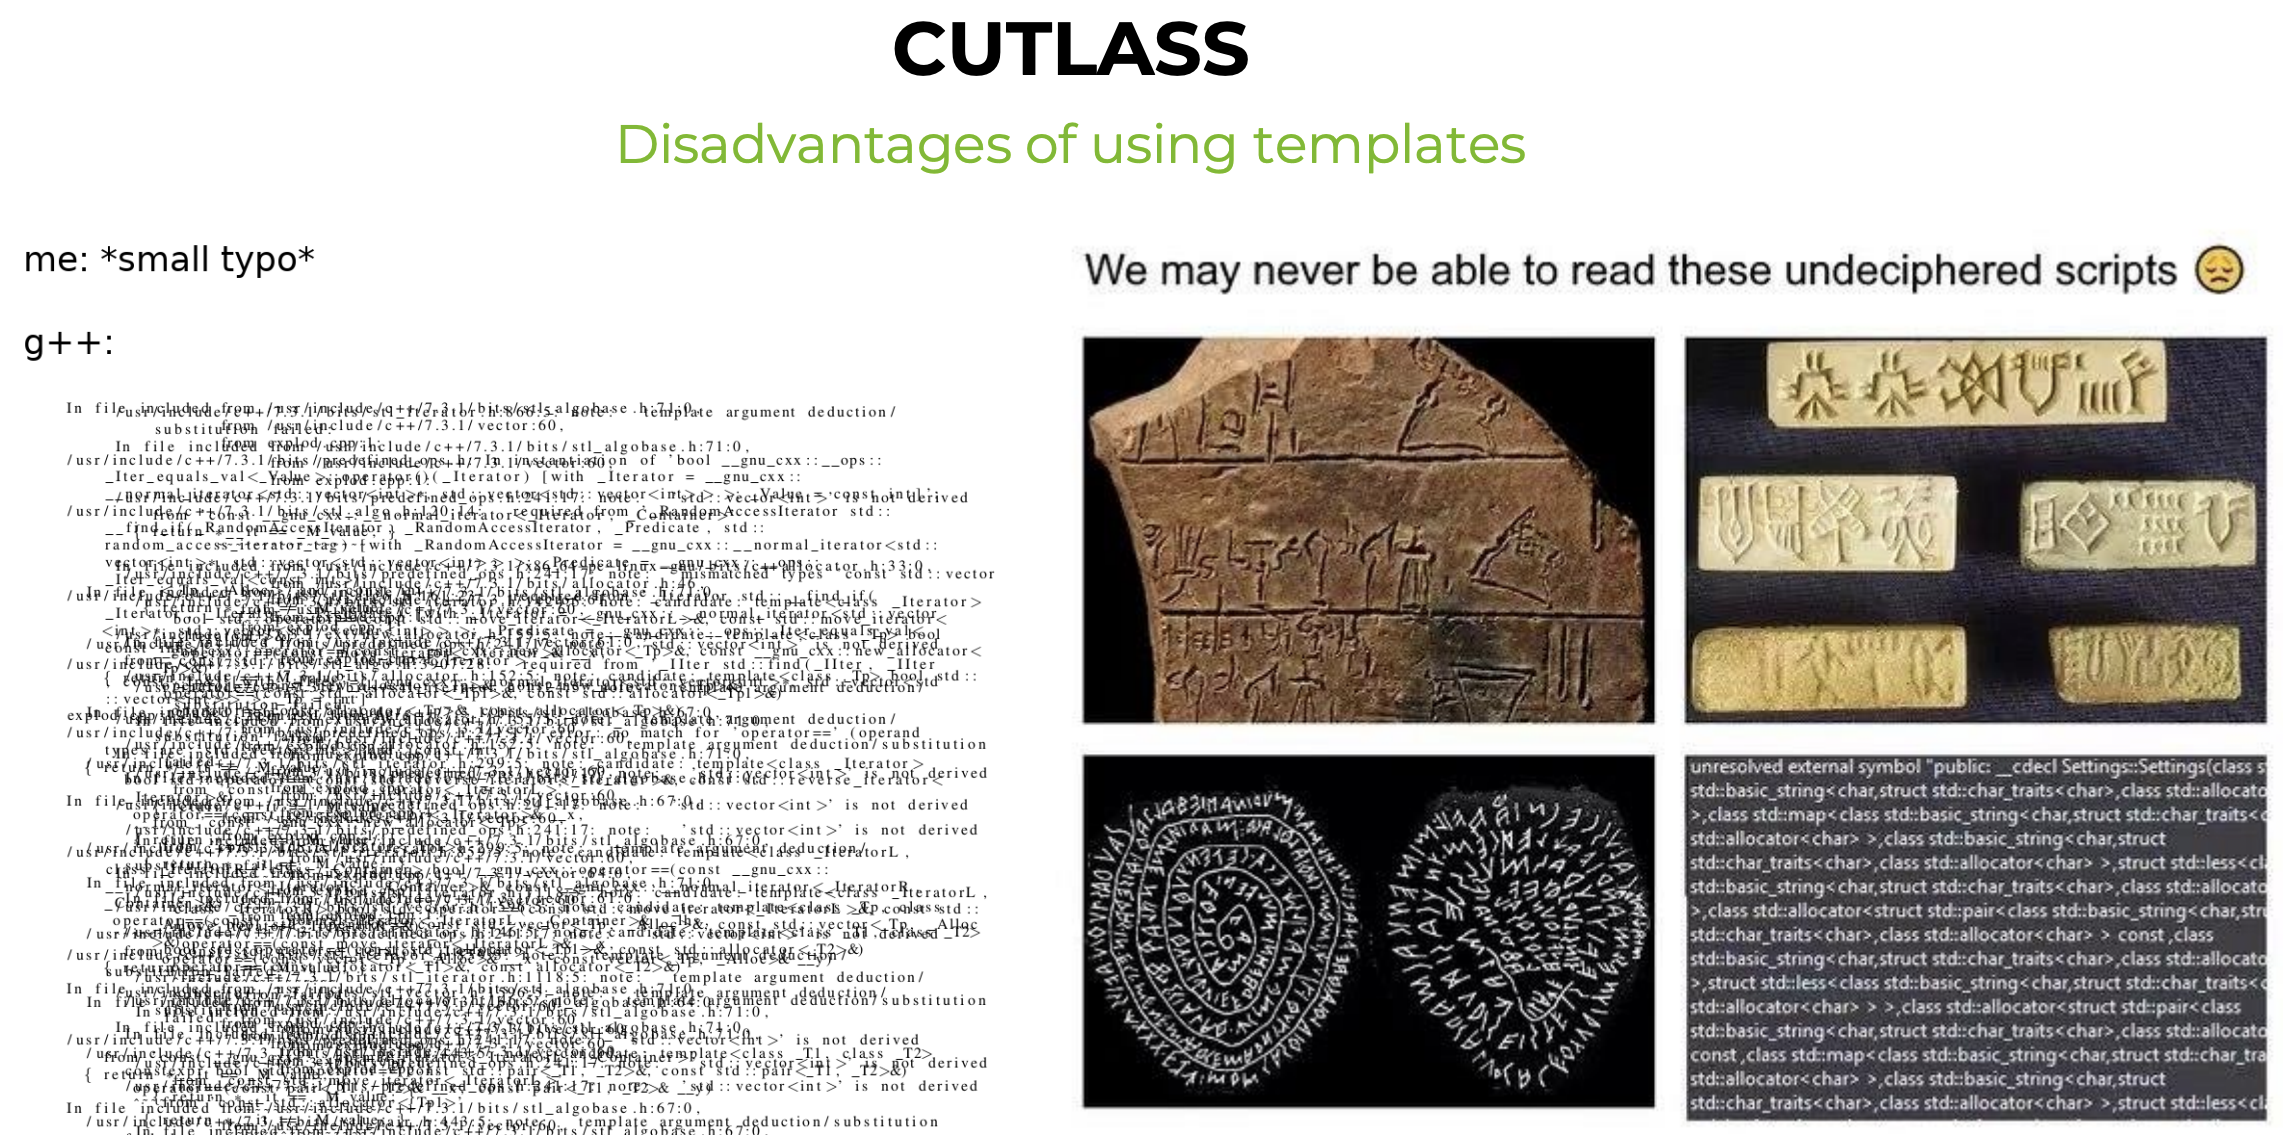
\includegraphics[width=0.8\textwidth]{day8_pm/img/2-templates}
		\caption{Cite: Yoolc's Sharing on CUTLASS}
	\end{figure}
\end{frame}

\subsection{Concurrency Support}
% 按时间引入 C++ 对并行编程的支持
% C++11:Threads, Mutual exclusion, Atomic operations, Condition variables, Futures
% C++20:Cooperative cancellation, Semaphores, Latches and Barriers
\begin{frame}[fragile]{Concurrency support library}
	\begin{itemize}
		\item \textbf{C++11} (We will learn):
		      \begin{itemize}
			      \item \texttt{<thread>}: Create and manage threads
			      \item \texttt{<mutex>}: Mutual exclusion for shared data
			      \item \texttt{<atomic>}: Atomic operations for thread safety
			      \item \texttt{<condition\_variable>}: Synchronization between threads
			      \item \texttt{<future>}: Asynchronous results
		      \end{itemize}
		\item \textbf{C++20}:
		      \begin{itemize}
			      \item \texttt{<stop\_token>}: Cooperative cancellation
			      \item \texttt{<semaphore>}, \texttt{<latch>}, and \texttt{<barrier>}: Advanced synchronization
		      \end{itemize}
	\end{itemize}
\end{frame}
